\documentclass[2pt, a4paper, fleqn]{extarticle}

\usepackage[T2A]{fontenc}
\usepackage[utf8]{inputenc}
\usepackage[english,russian]{babel}
\usepackage{url}
%\usepackage{pscyr}

%\renewcommand{\rmdefault}{ftm}
\usepackage{setspace}
\onehalfspacing

\usepackage{changepage}
\usepackage{indentfirst} %первый абзац
%%\usepackage{moreverb}
\usepackage[noend]{algorithmic}
\usepackage{amssymb, amsmath, multicol,amsthm}
%%
\usepackage{enumitem, multicol}
\usepackage{titleps,lipsum}
%%
\usepackage{mathrsfs}
\usepackage{verbatim}
\usepackage{pb-diagram}
\usepackage{graphicx}
\graphicspath{ {images/} }
\usepackage{wrapfig}
\usepackage{xcolor}
\definecolor{new}{RGB}{255,184,92}
\definecolor{news}{RGB}{112,112,112}
\usepackage{wallpaper}
\usepackage{float}
\usepackage{hyperref}
\hypersetup{
%colorlinks=true,%
%linkcolor=news,%
linkbordercolor=new,
}



\usepackage{geometry}
\geometry{top=1cm,bottom=2cm,left=1cm,right=1cm}

%\flushbottom
%\ruggedbottom

\binoppenalty=5000
\parindent=0pt

\newcommand{\EDS}{\ensuremath{\mathscr{E}}}
\newcommand*{\hm}[1]{#1\nobreak\discretionary{}%
{\hbox{$\mathsurround=0pt #1$}}{}}
\newcommand{\divisible}{\mathop{\raisebox{-2pt}{\vdots}}}
\renewcommand{\theequation}{\arabic{equation}}
\def\hm#1{#1\nobreak\discretionary{}{\hbox{$#1$}}{}}
\newcommand{\bbskip}{\bigskip \bigskip}



%%\DeclareMathOperator{\tg}{tg}
%%\DeclareMathOperator{\ctg}{ctg}

\let\leq\leqslant
\let\geq\geqslant



% Remove brackets from numbering in List of References
\makeatletter
\renewcommand{\@biblabel}[1]{\quad#1.}
\makeatother

\begin{document}

{\bf I.} \textit{Уравнение, решаемое на первом шаге расщепления:} $$\dfrac{\partial n_i}{\partial t} = \dfrac{\partial}{\partial z}\bigg[D\sin^2 I \bigg(\dfrac{\partial n_i}{\partial z}+\left(\dfrac{1}{T_p}\dfrac{\partial T_p}{\partial z}+\dfrac{1}{H}\right)n_i\bigg)-\dfrac{1}{a}D\sin I\cos I\left(\dfrac{\partial n_i}{\partial\varphi}+\dfrac{1}{T_p}\dfrac{\partial T_p}{\partial \varphi}n_i\right)\bigg]+[P-kn_i]$$


Во всех случаях используем для диффузионного слагаемого схему, получаемую применением формулы центральной разности дважды, а для потокового слагаемого $\dfrac{\partial}{\partial z} (un)$ центральную разность. Вычисление $u_\varphi$ ведётся по формуле $$u_\varphi \approx -\dfrac{1}{a}\cos I \sin I\dfrac{2}{n_{i, j+1}^t+n_{i, j-1}^t}\begin{cases}\dfrac{n_{i, j+1}^t-n_{i, j}^t}{\Delta\varphi}, \sin I \geq 0\\\dfrac{n_{i, j}^t-n_{i, j-1}^t}{\Delta\varphi}, \sin I \leq 0 .\end{cases}$$

Полная схема для уравнения на первом шаге: 

$$\dfrac{n_{i,j}^{t+1}-n_{i,j}^t}{\tau} = P - k n_{i, j}^{t+1} + \bigg[\left(D_{i+1/2}\dfrac{n_{i+1, j}^{t+1}-n_{i,j}^{t+1}}{h^2}-D_{i-1/2}\dfrac{n_{i,j}^{t+1}-n_{i-1,j}^{t+1}}{h^2}\right)+\left(\dfrac{u_{i+1}n_{i+1,j}^{t+1}-u_{i-1}n_{i-1,j}^{t+1}}{2h}\right) + MIX_{(z)i,j^{t, t+1}} \bigg]$$
Аппроксимация смешанной производной поясняется ниже.

На нижней границе $n_{i, j}^{t+1} = P/k$.

На граничных точках $\varphi = \pm 89{,}5^\circ$ коэффициент $\sin I$ перед смешанной производной мал. Для расчета в околополюсных точках из уравнения системы исключается слагаемое со смешанной производной:
$$\dfrac{n_{i,j}^{t+1}-n_{i,j}^t}{\tau} = P - k n_{i, j}^{t+1} + \bigg[\left(D_{i+1/2}\dfrac{n_{i+1, j}^{t+1}-n_{i,j}^{t+1}}{h^2}-D_{i-1/2}\dfrac{n_{i,j}^{t+1}-n_{i-1,j}^{t+1}}{h^2}\right)+\left(\dfrac{u_{i+1}n_{i+1,j}^{t+1}-u_{i-1}n_{i-1,j}^{t+1}}{2h}\right) \bigg]$$


\bigskip

{\bf II.} \textit{Уравнение, решаемое на втором шаге расщепления:}

$$\dfrac{\partial n}{\partial t} = \dfrac{1}{a\cos\varphi} \dfrac{\partial }{\partial \varphi}\left[\dfrac{D}{a}\cdot(\cos^2  I \cos\varphi)\cdot\dfrac{\partial n}{\partial \varphi}-D\cdot(\sin I\cos I\cos\varphi)\cdot \dfrac{\partial n}{\partial z} - u\cdot(\sin I \cos I \cos\varphi)\cdot n \right]$$

Здесь $u = D\left(\dfrac{1}{T_p}\dfrac{\partial T_p}{\partial z}+\dfrac{1}{H}\right)$~---~эффективная скорость из первого шага, $I = \arctg(2\tg \varphi)$.

В качестве начальных условий выступает решение уравнения с первого шага расщепления. Введём две функции: $$A(\varphi) = \cos \varphi \cdot \cos^2(\arctg(2\tg \varphi)) = \dfrac{\cos\varphi}{1+4\tg^2\varphi}\mbox{ и }B(\varphi) = \cos\varphi \cdot \sin(2\arctg(2\tg \varphi))=\dfrac{4\sin\varphi}{1+4\tg^2\varphi}.$$

С помощью этих функций задачу можно переписать в следующем виде: 
$$\dfrac{\partial n}{\partial t} = \dfrac{1}{\cos\varphi} \dfrac{\partial }{\partial \varphi}\left[\dfrac{D}{a^2}A(\varphi)\dfrac{\partial n}{\partial \varphi}-\dfrac{D}{2a}B(\varphi) \dfrac{\partial n}{\partial z} - \dfrac{u}{2a}B(\varphi) n \right]$$

Для полного уравнения используем следующую схему:
$$\dfrac{n_{i,j}^{t+1}-n_{i,j}^t}{\tau} = \dfrac{1}{\cos\varphi_j} \bigg[\dfrac{D}{a^2}\left(A(\varphi_{j+1/2})\dfrac{n_{i, j+1}^{t+1}-n_{i,j}^{t+1}}{\Delta\varphi^2}-A(\varphi_{j-1/2})\dfrac{n_{i,j}^{t+1}-n_{i,j-1}^{t+1}}{\Delta\varphi^2}\right)-$$ $$-\dfrac{u}{2a}\left(\dfrac{B(\varphi_{j+1})n_{i,j+1}^{t+1}-B(\varphi_{j-1})n_{i,j-1}^{t+1}}{2\Delta\varphi}\right) - MIX_{\varphi}(n)_{i, j}^{t+1} \bigg]$$

Здесь $MIX_{\varphi}(n)_{i, j}^{t+1}$~---~аппроксимация смешанной производной.

\bigskip
\newpage

{\bf III.} \textit{Аппроксимация смешанной производной.}

Рассмотрим на примере смешанной производной в уравнении второго шага расщепления аппроксимацию второго порядка по пространству: для смешанной производной $-\dfrac{D}{2a\cos\varphi}\dfrac{\partial}{\partial\varphi}\left(B(\varphi)\dfrac{\partial n}{\partial z}\right)$ запишем следующие четыре аппроксимации (здесь $B_j \equiv B(\varphi_j)$: 

$$-\dfrac{D}{2a\cos\varphi}\dfrac{\partial}{\partial\varphi}\left(B(\varphi)\dfrac{\partial n}{\partial z}\right) \approx $$ $$\approx-\dfrac{D}{2ah\Delta\varphi \cos\varphi_j} \begin{cases}  B_{j+1} n_{i, j+1}^{t+1} - B_jn_{i, j}^{t+1} - B_{j+1}n_{i-1, j+1}^t + B_j n_{i-1, j}^t \mbox{, справедливо при } B(\varphi_j) < 0 \mbox{, схема (1);}\\ B_{j+1}n_{i+1, j+1}^t - B_j n_{i+1, j}^t - B_{j+1}n_{i, j+1}^{t+1}+B_j n_{i, j}^{t+1}\mbox{, справедливо при } B(\varphi_j) > 0 \mbox{, схема (2);} \\ B_j n_{i,j}^{t+1} - B_{j-1}n_{i, j-1}^{t+1} - B_j n_{i-1, j}^t + B_{j-1}n_{i-1, j-1}^t\mbox{, справедливо при } B(\varphi_j) > 0 \mbox{, схема (3);} \\ B_{j+1}n_{i+1, j+1}^t - B_j n_{i+1, j}^t - B_{j+1}n_{i, j+1}^{t+1} + B_{j}n_{i, j}^{t+1}\mbox{, справедливо при } B(\varphi_j) < 0 \mbox{, схема (4).}\end{cases}$$ 

Первый вариант схемы первого порядка: при $B(\varphi) \geq 0$ (т.~е. в верхнем полушарии) вычисление ведется по формуле (3), а в нижнем полушарии, при $B(\varphi) \leq 0$, соответственно, по формуле (1).

Второй вариант схемы первого порядка: при $B(\varphi) \geq 0$ (т.~е. в верхнем полушарии) вычисление ведется по формуле (2), а в нижнем полушарии, при $B(\varphi) \leq 0$, соответственно, по формуле (4).

Для получения схемы второго порядка по пространству используем аппроксимации, рассмотренные в предыдущем пункте: если $B(\varphi) \geq 0$, то аппроксимируем смешанную производную полусуммой аппроксимаций (2) и (3), иначе~---~полусуммой (1) и (4). Для вычисления в околополюсных точках отождествляем необходимые точки вне расчетной области с симметричными им относительно полюсов. 

\bigskip

{\bf IV.} \textit{Различные аппроксимации верхнего граничного условия для уравнения, решаемого на первом шаге расщепления.}

На верхней границе $z = z_{ub} = 500$~км ставится условие постоянства полного потока $$D\sin^2 I\dfrac{\partial n}{\partial z} + u\sin^2 I n - \dfrac{1}{a}D\sin I \cos I \dfrac{\partial n}{\partial \varphi} = F_{ub},$$ константа $F_{ub}$ полагается малой и при расчетах приравнивается к нулю.

Рассмотрим следующие четыре варианта аппроксимации этого граничного условия:

\begin{itemize}

\item[Схема 0.] В предположении малости влияния смешанной производной на верхней границе на решение в граничном условии производная по $\varphi$ отбрасывается.

В численных экспериментах такой подход показал плохие результаты: помимо жестких ограничений на шаг по времени для устойчивости, характер численного решения существенно отличается от соответствующего решения задачи без смешанных производных (сеточное решение задачи без смешанных производных приведено ниже).

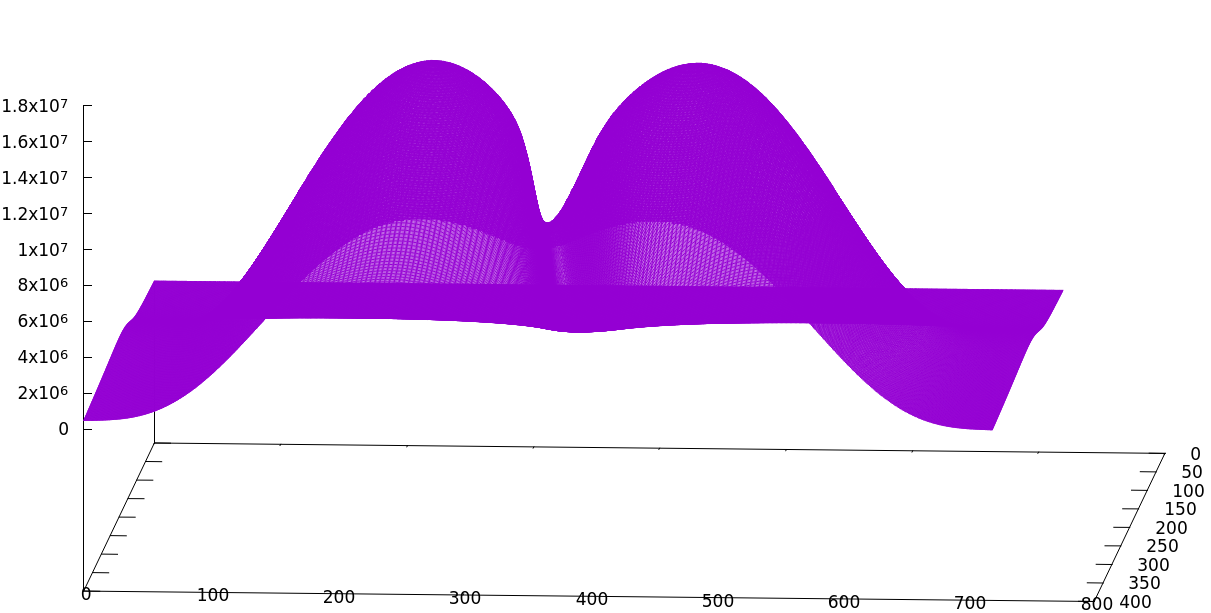
\includegraphics[scale=0.3]{scheme0.png}

\item[Схема 1.] В тех же предположениях при расчетах на верхней границе в полусуммах по квадратам полностью зануляются те квадраты, что содержат узлы вне расчетной области.

Расчеты по данной схеме при малых шагах по пространству провести затруднительно, даже при шагах по времени порядка нескольких секунд схема неустойчива (на пространственной сетке $\Delta\varphi = 0{,}25^\circ$, $h = 1$~км).

Результат расчета на грубой сетке $\Delta\varphi = 1^\circ$, $h = 5$~км) приведен ниже. Характер сеточного решения близок к результату расчета по предыдущей схеме.

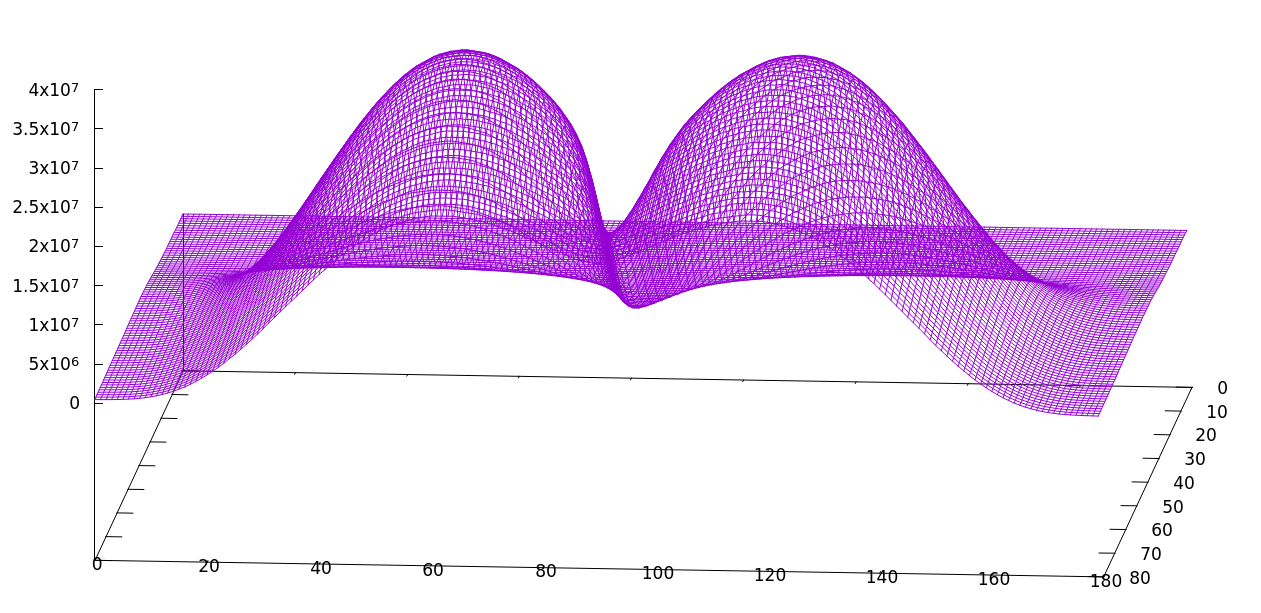
\includegraphics[scale=0.3]{scheme1.png}

\item[Схема 2.] Проинтегрируем наше уравнение по прямоугольнику, вершинами которого являются четыре центра соседних ячеек: пара выше $z = z_{ub}$, а вторая пара ниже: $$\int_{\varphi_{j-1/2}}^{\varphi_{j+1/2}}\int_{h_{N-1/2}}^{h_{N+1/2}} \dfrac{\partial}{\partial z}(...)dzd\varphi = \int_{\varphi_{j-1/2}}^{\varphi_{j+1/2}} \bigg[F - D_{N-1/2}\sin^2 I\left(\dfrac{\partial}{\partial z}\right)_{N-1/2}-u_{N-1/2}n_{N-1/2}\sin^2 I + $$ $$+ \dfrac{1}{2a}D_{N-1/2}\sin(2I)\left(\dfrac{\partial}{\partial \varphi}\right)_{N-1/2}\bigg]d\varphi \approx F\Delta\varphi - D_{N-1/2}\sin^2 I_j\Delta\varphi \left(\dfrac{\partial n}{\partial z}\right)_{N-1/2} - $$ $$-u_{N-1/2}n_{N-1/2, j}\Delta\varphi + \dfrac{1}{2a}D_{N-1/2}\sin(2I_j)(n_{N-1/2, j+1/2}-n_{N-1/2, j-1/2}) = \int_{\varphi_{j-1/2}}^{\varphi_{j+1/2}}\int_{h_{N-1/2}}^{h_{N+1/2}} \dfrac{\partial}{\partial t} = \Delta\varphi \cdot h \cdot \dfrac{\partial n}{\partial t}.$$
Затем полагаем $$\left(\dfrac{\partial n}{\partial z}\right)_{N-1/2, j} = \dfrac{n_{N, j}-n{N-1, j}}{h};$$ $$u_{N-1/2}n_{N-1/2} = \dfrac{1}{2}(u_Nn_N + u_{N-1}n_{N-1}),$$ а также $$n_{N-1/2, j+1/2}-n_{N-1/2, j-1/2} = \dfrac{1}{4}(n_{N, j+1}+n_{N, j}+n_{N-1, j+1}+n_{N-1, j}-n_{N, j}-n_{N, j-1}-n_{N-1, j}-n_{N-1, j-1}) = $$ $$=\dfrac{1}{4}(n_{N, j+1}+n_{N-1, j+1}-n_{N, j-1}-n_{N-1, j-1})$$

Условие устойчивости схемы~---~наиболее жесткое из рассматриваемых трёх схем. Результаты расчета на грубой сетке приведены на графике.

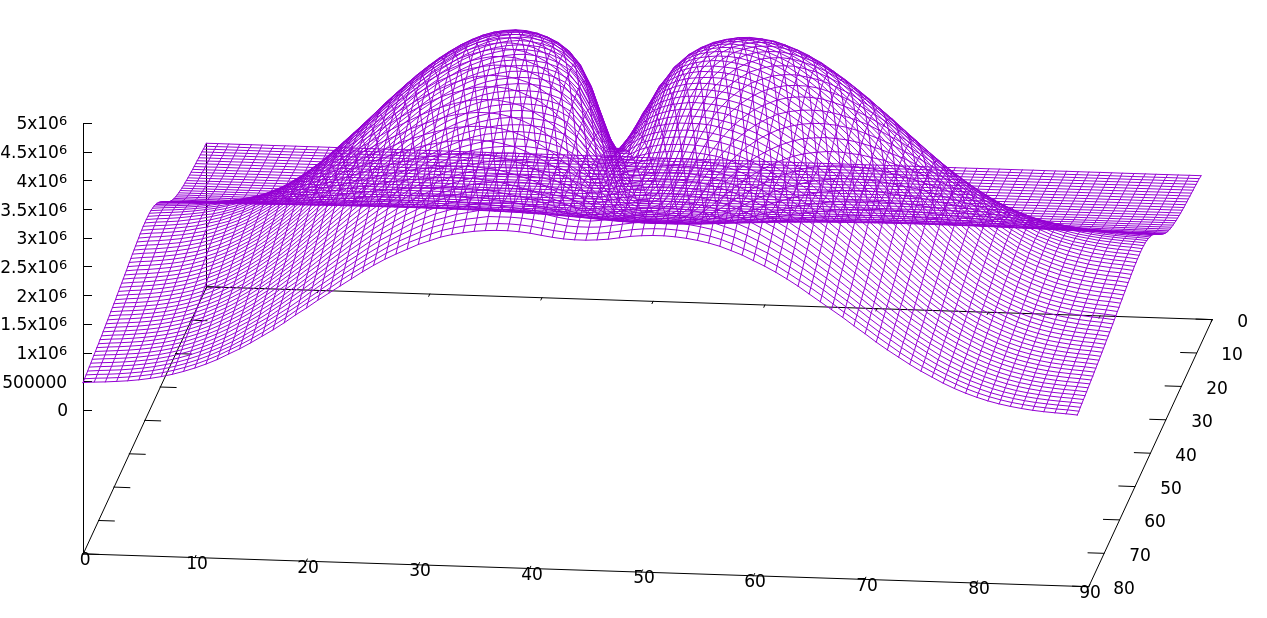
\includegraphics[scale=0.3]{scheme2.png}

\item[Схема 3.] Заметим, что при расчетах смешанной производной по узлам~---~вершинам четырех квадратов получаемые схемы в рамках каждого квадрата имеют вид <<(разность на верхней стороне квадрата) - (разность на нижней стороне квадрата)>>. При этом разность на верхней стороне квадрата аппроксимирует $\dfrac{\partial n}{\partial\varphi}$ в центре верхней стороны.

Зададим знак коэффициента перед смешанной производной. При этом сама производная в центральном узле аппроксимируется полусуммой производных в центрах двух квадратов, центрально симметричной относительно центрального узла. Граничное условие, включающее обнуление $\left(\dfrac{\partial n}{\partial\varphi}\right)_{N+1/2}$ можно аппроксимировать согласованно со схемой, приравняв нулю полусумму двух разностей на верхних сторонах двух используемых квадратов.

Получающаяся схема имеет большой запас устойчивости (даже при отсутствии  монотонизатора, обнуляющего все возникающие отрицательные значения концентрации), а характер численного решения наиболее близок к результату расчетов в задаче без смешанных производных.

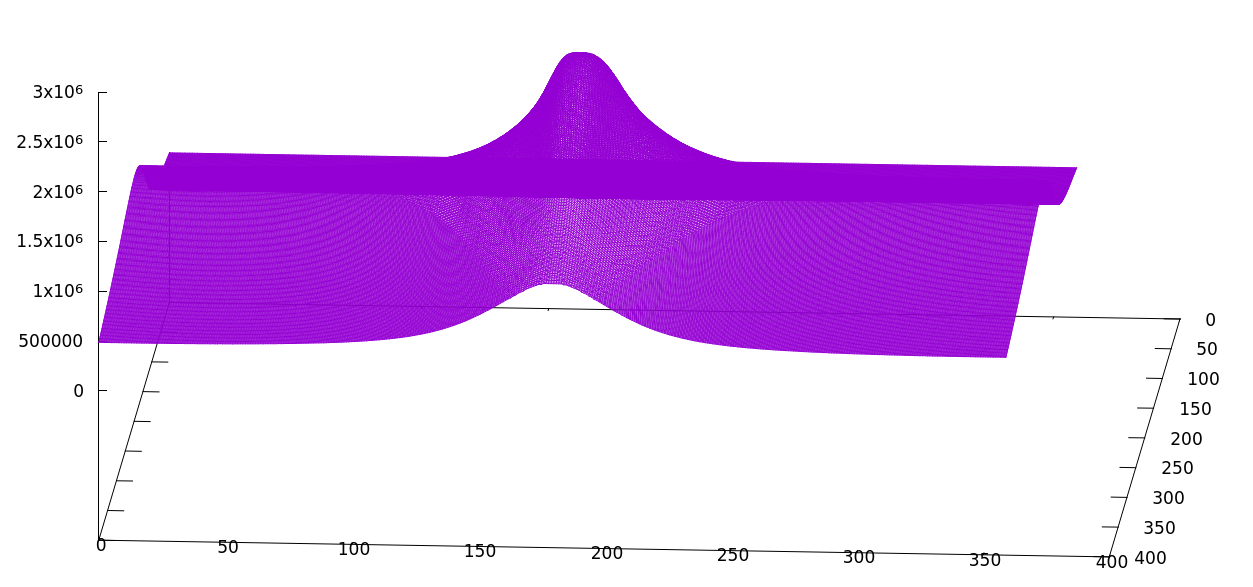
\includegraphics[scale=0.3]{scheme3.png}

\end{itemize}

{\bf V.} \textit{Задача без смешанной производной.}

Рассматривается уравнение, решаемое на втором шаге расщепления, без учёта смешанной производной: $$\dfrac{\partial n}{\partial t} = \dfrac{1}{a\cos\varphi} \dfrac{\partial }{\partial \varphi}\left[\dfrac{D}{a}\cdot(\cos^2  I \cos\varphi)\cdot\dfrac{\partial n}{\partial \varphi} - u\cdot(\sin I \cos I \cos\varphi)\cdot n \right] =  \dfrac{1}{\cos\varphi} \dfrac{\partial }{\partial \varphi}\left[\dfrac{D}{a^2}A(\varphi)\dfrac{\partial n}{\partial \varphi} - \dfrac{u}{2a}B(\varphi) n \right].$$

Результат расчета стационарного решения приведен на графике:

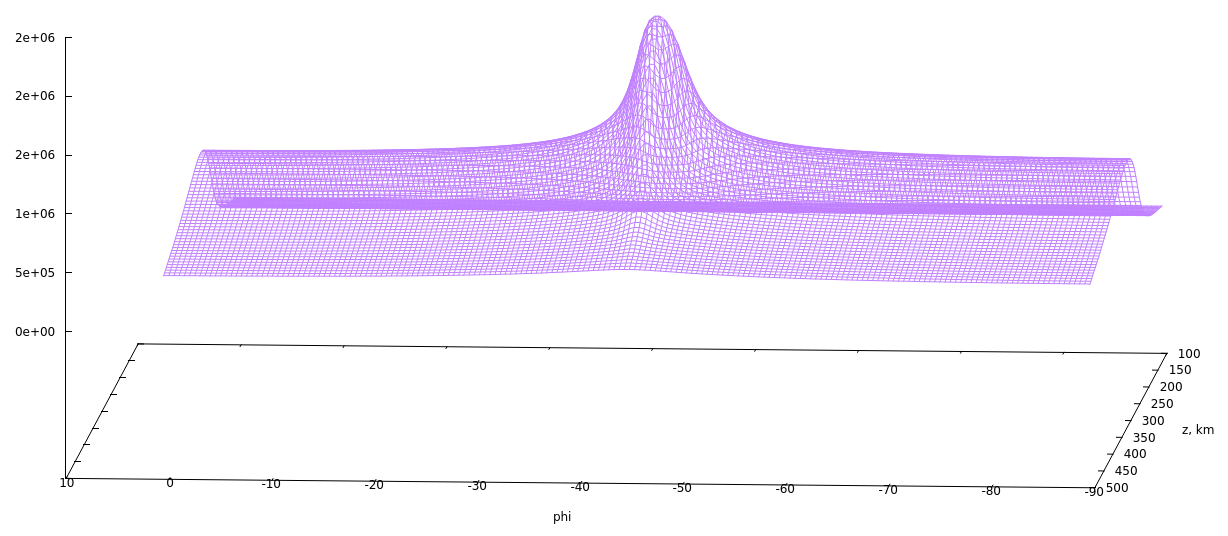
\includegraphics[scale=0.5]{linear_2st_order}

\newpage

{\bf VI.} \textit{Суточный ход и исследование сходимости сеточного решения при уменьшающихся значениях шага по времени.}

Проведен следующий эксперимент: на фиксированной сетке по пространству выполняется расчет на два дня при постоянном дневном значении фотоионизации, а затем с полученного сеточного решения, взятого в качестве начальных данных, проводятся параллельно два расчета суточного хода с различными шагами по времени: $\tau$ и $\tau_1 = \tau/2$. Вычисляется $\mathbb{L}_1$-норма сеточного решения (сеточный аналог тройного интеграла по всей расчетной области и по всему рассматриваемому временному отрезку), а также $\mathbb{L}_1$-норма разности сеточных решений с рассматриваемыми двумя шагами по времени.

Полученные результаты приведены в таблице. Расчет показывает, что относительная ошибка $\varepsilon$ даже на грубых сетках не превосходит $\approx 10^{-3}$, что оправдывает применимость метода расщепления к рассматриваемой задаче.

\smallskip

\begin{center}
\begin{tabular}{|c|c|c|c|}
\hline
$\tau$&$||n||_{\mathbb{L}_1}$&$||err||_{\mathbb{L}_1}$&$\varepsilon$\\
\hline
150&28155097.5393827&85023.4523162335&0.003\\
\hline
100&42202367.4996776&86547.3785379812&0.0021\\
\hline
50&84344183.7824046&88609.8117758545&0.0011\\
\hline
10&421478366.158547&91848.4416168127&0.00021\\
\hline
5&842896083.238167&92622.2986773716&0.00011\\
\hline
1&4214237864.15977&93471.0498304002&0,000022\\
\hline
\end{tabular}
\end{center}
\end{document}



